    
    \begin{frame}{Dane jako zasób strategiczny}
    \begin{alertblock}{Dlaczego dane są cenne?}
        \begin{itemize}
          \item Dane to nowa forma kapitału - porównywalna z ropą czy złotem.
          \item Pozwalają przewidywać zachowania i wpływać na decyzje.
          \item Są gromadzone masowo przez wiele podmiotów.
        \end{itemize}
    \end{alertblock}
    \end{frame}
    
    
    \begin{frame}{Firmy reklamowe i technologiczne}
    \begin{columns}[c]
        \column{.5\textwidth}
        \begin{alertblock}{Profilowanie i personalizacja}
            \begin{itemize}
              \item Dane z aktywności online służą do budowy profili.
              \item Użytkownik otrzymuje „spersonalizowaną rzeczywistość”.
              \item Reklamy, ceny, treści - wszystko dostosowane do profilu. \cite{EFF}
            \end{itemize}
        \end{alertblock}
        \column{.5\textwidth}
        \begin{figure}
          \centering
          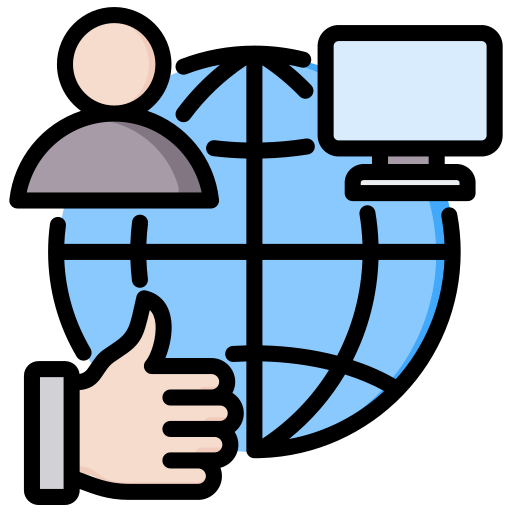
\includegraphics[height=0.45\textheight]{images/social-network.png}
        \end{figure}
    \end{columns}
    \end{frame}
    
    
    \begin{frame}{Pracodawcy i uczelnie}
    \begin{alertblock}{Decyzje oparte na danych}
        \begin{itemize}
          \item Dane z mediów społecznościowych mogą wpłynąć na decyzję o zatrudnieniu.\cite{DIGITAL_GLOBAL}
          \item Platformy e-learningowe śledzą aktywność studentów.
          % \item Uczelnie analizują zaangażowanie, postępy, a nawet emocje.
        \end{itemize}
    \end{alertblock}
    \end{frame}
    
    
    \begin{frame}{Instytucje państwowe i służby}
    \begin{columns}[c]
        \column{.5\textwidth}
        \begin{figure}
          \centering
          
\includegraphics[height=0.45\textheight]{images/user-management.png}
        \end{figure}
        \column{.5\textwidth}
        \begin{alertblock}{Zarządzanie i kontrola}
            \begin{itemize}
              \item Dane wykorzystywane są do nadzoru i przewidywania ryzyk.
              \item W Chinach działają systemy oceny obywateli.\cite{DIGITAL_LOCAL}
              \item W wielu krajach zbierane są dane z kamer, mediów i smartfonów.
            \end{itemize}
        \end{alertblock}
    \end{columns}
    \end{frame}
    
    
    \begin{frame}{Firmy ubezpieczeniowe i banki}
    \begin{alertblock}{Ryzyko obliczane danymi}
        \begin{itemize}
          \item Twoje nawyki zakupowe i lokalizacja wpływają na ocenę ryzyka.
          \item Styl jazdy może zwiększyć lub obniżyć składkę ubezpieczenia.
        \end{itemize}
    \end{alertblock}
    \end{frame}
    
    
    \begin{frame}{Cyberprzestępcy}
    \begin{columns}[c]
        \column{.5\textwidth}
        \begin{figure}
          \centering
          
\includegraphics[height=0.45\textheight]{images/firewall.png}
        \end{figure}
        \column{.5\textwidth}
        \begin{alertblock}{Kto jeszcze się interesuje danymi?}
            \begin{itemize}
              \item Skradzione dane mogą zostać odsprzedane lub wykorzystane do szantażu.
              \item Phishing, kradzież tożsamości, podrabiane profile.\cite{PHISHING_REPORT}
              \item Często wykorzystywane są dane z przecieków publicznych.
            \end{itemize}
        \end{alertblock}
    \end{columns}
    \end{frame}
    
    \begin{frame}{Komu ufamy z naszymi danymi?}
    \begin{alertblock}{Zostawiamy więcej, niż nam się wydaje}
        \begin{itemize}
          \item Nie wiemy, kto analizuje i przetwarza nasze dane.
          \item Coraz trudniej uniknąć śledzenia, nawet jeśli „nic nie udostępniamy”.
          \item Dane osobowe są paliwem cyfrowego świata - i zagrożeniem, i wartością.
        \end{itemize}
    \end{alertblock}
    \end{frame}